\documentclass[letterpaper, 12pt]{texMemo}
\usepackage[american]{babel}
\usepackage{graphicx}
\usepackage{caption}
\usepackage[citestyle=apa,style=apa,backend=biber]{biblatex}
\captionsetup{justification = raggedright, singlelinecheck = false}
\DeclareLanguageMapping{american}{american-apa}
\addbibresource{bibliography.bib}
\memoto{Dr. William Hsu}
\memofrom{Blair Urish}
\memosubject{Visual Aids}
\memodate{February 27, 2017}

\begin{document}
\maketitle
\begin{flushleft}
\subsection*{Introduction}
The purpose of this memo is to provide examples of two visual aids that will be used in this literature review. Justifications for the inclusion of the visual aids is also given.

\subsection*{Figure 1}
This figure identifies the three layers of the Internet of Things architecture. The figure provides the reader with examples of services that function at each layer.


\begin{figure}[h!]
	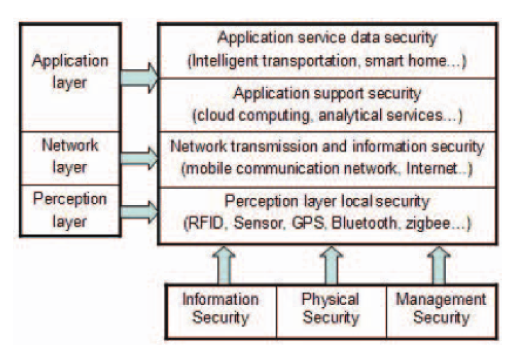
\includegraphics[width=\linewidth]{figure2.png}
	\caption{Internet of Things Architecture}
	\label{fig:arch}
\end{figure}

\subsection*{Justification for Figure 1}
It is important for the reader to understand the differences between each of the layers of the Internet of Things Architecture. 
This figure provides examples of devices commonly found in each layer and what type of security is necessary. 

\subsection*{Figure 2}
This figure shows the current communication standards that can be applied to each layer of the IoT architecture. 

\begin{figure}[h!]
	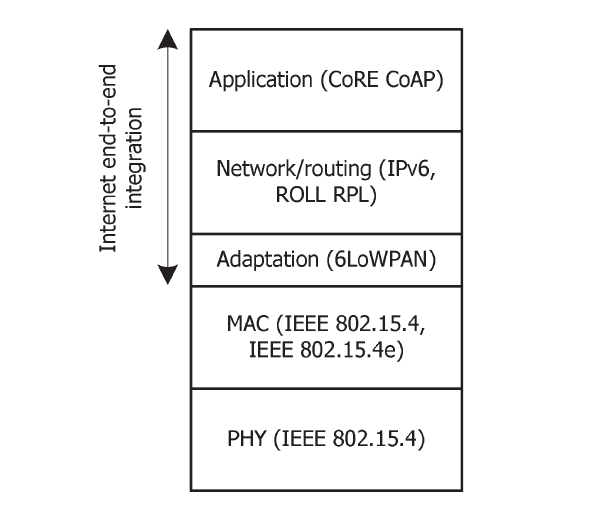
\includegraphics[width=\linewidth]{figure3.png}
	\caption{Internet of Things Communication Standards}
	\label{fig:arch}
\end{figure}

\subsection*{Justification for Figure 2}
In the final report, all of the standards in the above figure will be discussed in detail. Having this figure in the report will allow readers to quickly see what standards
will be addressed and what layer they apply to. 

\newpage
Bibliography\\
~\newline
\fullcite{Zhao6746513}\\
~\newline
\fullcite{Granjal7005393}
\end{flushleft}
\end{document}
